\section{理论推导}

\subsection{复现的物理模型}

复现围绕两个物理场景：\textbf{单球散射}（Fig.~1/2，有 Lorenz--Mie 解析真值可做独立基准）与\textbf{耦合双金盘}（Fig.~3，无解析解，需数值求解）。

\begin{figure}[H]
\centering
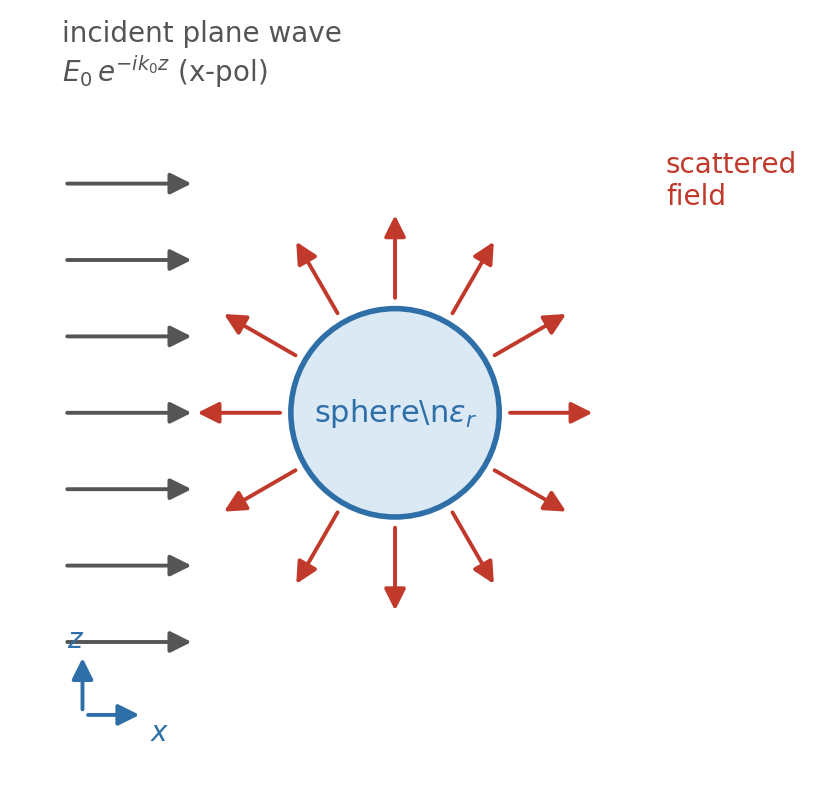
\includegraphics[width=0.74\textwidth]{figs/schematic_sphere.png}
\caption{物理场景一：平面波 $E_0\,e^{-ik_0 z}$（$x$ 偏振）入射到半径为 $a$ 的单球，散射出辐射场。Fig.~1 用介电球 $\varepsilon_r=6.25$，Fig.~2 用金球（Johnson--Christy 色散）。}
\label{fig:schematic_sphere}
\end{figure}

\begin{figure}[H]
\centering
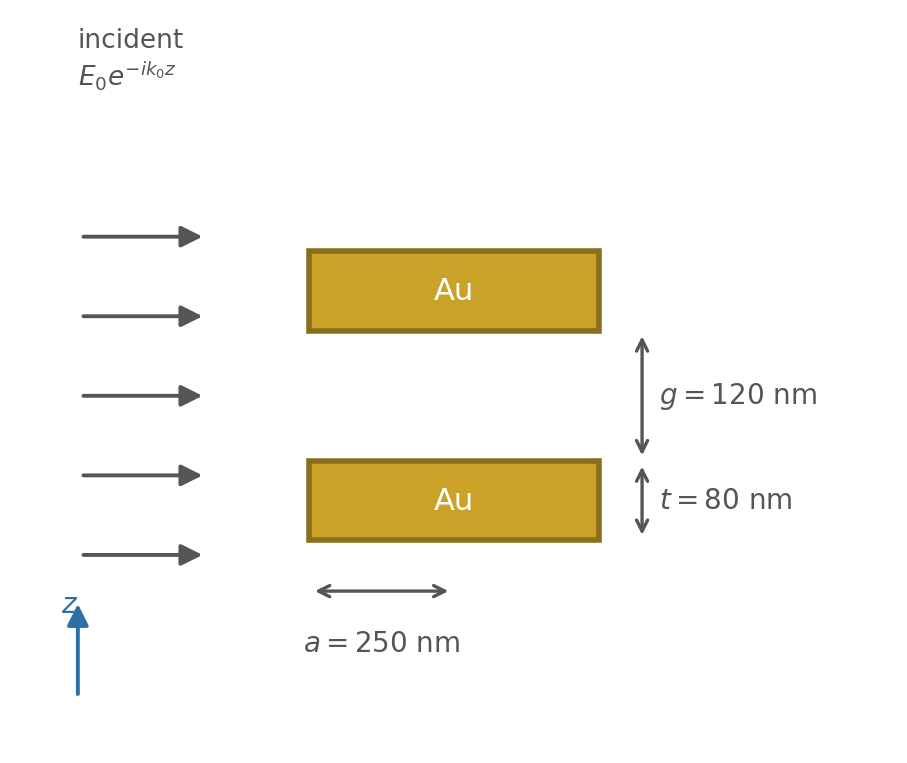
\includegraphics[width=0.64\textwidth]{figs/schematic_double_disk.png}
\caption{物理场景二：两个耦合金纳米盘，半径 $a=250$ nm、高 $t=80$ nm、间隙 $g=120$ nm。Fig.~3 无解析解，用 COMSOL 频域有限元（FEM）与边界元（BEM）两种求解器交叉验证。}
\label{fig:schematic_double_disk}
\end{figure}

\subsection{四篇论文的理论链}

按「从 Maxwell 到精确多极展开」的顺序，四篇论文构成一条理论链：

\begin{enumerate}
  \item \textbf{Grahn 2012}：从 Maxwell 方程出发，把任意局域电流分布 $\mathbf J(\mathbf r)$ 展开为电流多极矩，并给出电流多极矩到散射场多极系数 $a_E(l,m), a_M(l,m)$ 的映射（Eq.~(1)--(16)）。这是后续工作的出发点。
  \item \textbf{Fernandez-Corbaton 2015}：长波近似下偶极矩定义不唯一，给出局域电流分布的\textbf{精确}电偶极矩（保留全部 $kr$ 阶），揭示偶极展开里的 toroidal 项。
  \item \textbf{Fernandez-Corbaton 2017}：严格证明 toroidal 多极\textbf{不是独立自由度}——电部分与 toroidal 部分各自含不可观测的非辐射分量，求和才抵消；toroidal 只是电偶极系数对电磁尺寸展开的高阶修正。
  \item \textbf{Alaee 2018}：推广到全部多极阶。Table 1 是长波近似（$kr\to0$ 截断），Table 2 是保留球 Bessel 函数 $j_l(kr)$ 的精确表达式；Table 1 是 Table 2 的 $kr\to0$ 极限。
\end{enumerate}

这条理论链的关键公式如下。\textbf{Table 1（长波近似）}给出熟知的偶极/磁偶极矩：
\[
p_\alpha = \int P_\alpha\,dV,\qquad
m_\alpha = \frac{i\omega}{2}\int (\mathbf r\times\mathbf P)_\alpha\,dV,
\]
其中 $\mathbf P$ 是极化场，电偶极散射贡献里还有 toroidal 项（$k^2/10$ 修正）。\textbf{Table 2（精确）}保留球 Bessel 核，例如精确电偶极矩的积分核为 $j_1(kr)/(kr)$；退化检查的关键是 $j_l(kr)/(kr)^l\to1/(2l+1)!!$，使 Table 2 在 $kr\to0$ 退化回 Table 1。\textbf{Grahn 2012} 的电流多极矩到散射系数的映射常数为
\[
C_1=-\frac{ik^3}{6\pi E_0},\qquad
C_2=-\frac{k^4}{60\pi E_0},\qquad
C_3=-\frac{ik^5}{210\pi E_0}
\]
（对应正文 Eq.~(35)--(48)）。

\subsection{矢量球谐的推导}

我手推了从 Maxwell 到 Grahn Eqs.~(1)--(16) 的矢量球谐（VSH）展开链，约 66 页笔记，逐步不跳步。矢量球谐的定义是
\[
\mathbf M_{lm} = \frac{1}{\sqrt{l(l+1)}}\nabla\times(\mathbf r\,Y_{lm}),\qquad
\mathbf N_{lm} = \frac{1}{k}\nabla\times\mathbf M_{lm},
\]
它们满足正交完备性，是任意场/电流投影到多极分量的基。核心路径：

\[
\text{Maxwell 方程} \;\longrightarrow\; \text{矢量球谐 } \mathbf M_{lm},\mathbf N_{lm} \;\longrightarrow\; \text{Mie 严格解} \;\longrightarrow\; \text{多极投影} \;\longrightarrow\; \text{电流多极矩映射}
\]

三个关键节点：

\begin{itemize}
  \item \textbf{矢量球谐的正交完备性}：$\mathbf M_{lm},\mathbf N_{lm}$ 在球面上正交，这是把任意场/电流投影到多极分量的数学基础；用球面谐函数 $Y_{lm}$ 的梯度与旋度显式构造。
  \item \textbf{散射电流到多极系数的投影}：散射电流 $\mathbf J(\mathbf r)$ 与 $\mathbf M_{lm},\mathbf N_{lm}$ 做内积，分部积分把体积分化为含 $j_l(kr)$ 核的积分——这正是 Table 2 的 Bessel 核来源。
  \item \textbf{长波退化的来源}：$j_l(kr)\xrightarrow{kr\to0}(kr)^l/(2l+1)!!$，代入后 Table 2 逐条退化回 Table 1，toroidal 项（ED 的 $k^2/10$ 项）自动显现为 $j_2/(kr)^2\to1/15$ 的极限。
\end{itemize}

\subsection{推导中的验证}

两类验证，避免「公式抄对但系数抄错」：

\begin{enumerate}
  \item \textbf{scipy 数值验证}：对关键积分核与投影结果，用 scipy 的球 Bessel 函数、Legendre 多项式独立数值计算，与手推解析系数逐点比对，锁定系数（ED 的 $3$、MQ 的 $15$ 都由退化验证固定）。
  \item \textbf{退化检查}：系统检查 Table 2 在 $kr\to0$ 逐条退化回 Table 1（ED/MD/EQ/MQ），并验证 $j_l/(kr)^l\to1/(2l+1)!!$ 的系数（$1/3, 1/15, 1/105$）。
\end{enumerate}

\begin{important}
  \textbf{可信的依据}：一条公式链从 Maxwell 出发、经多次分部积分与投影，中间任何一步系数错都会在退化检查里暴露。Table 2 $\to$ Table 1 的逐条退化 + scipy 独立数值比对，构成「内部一致性」与「外部独立」双重校验。
\end{important}

完整逐步推导见推导笔记 \url{https://github.com/PKU-QNO/optics-agent-zyz/blob/main/MIE-0814/reports/vector-multipole-derivation.pdf}。代数化简与公式核对部分借助了 AI 辅助，推导逻辑与退化检查独立完成并逐一验证。
